\documentclass[12pt]{report}

\usepackage{parskip}
\usepackage[utf8]{inputenc}
\usepackage{graphicx}
\usepackage{titlesec}
\usepackage{listings}
\usepackage{hyperref}
\usepackage[toc]{glossaries}
\usepackage[margin=1in]{geometry}

% Start new page after section
\newcommand{\sectionbreak}{\clearpage}

\titleformat{\chapter}[display]
  {\normalfont\huge\bfseries}{}{0pt}{\Huge}
\titlespacing*{\chapter}
  {0pt}{10pt}{40pt}

\title{
	{Netværkseksamen}\\
}

\author{
\input{author}
}

\renewcommand{\contentsname}{Indholdsfortegnelse}

\date{
\input{date}
}

\begin{document}
\maketitle

\tableofcontents

\chapter{Networks: Protocols, Layers}
\section{Internet overblik}

\subsection{Introduktion}
\begin{itemize}
	\item Hosts, end systems (Client, Server)
	\item Packets
	\item Communication links
	\item Packet switches
	\item Internet Service Providers (ISP)
	\item Route
\end{itemize}

{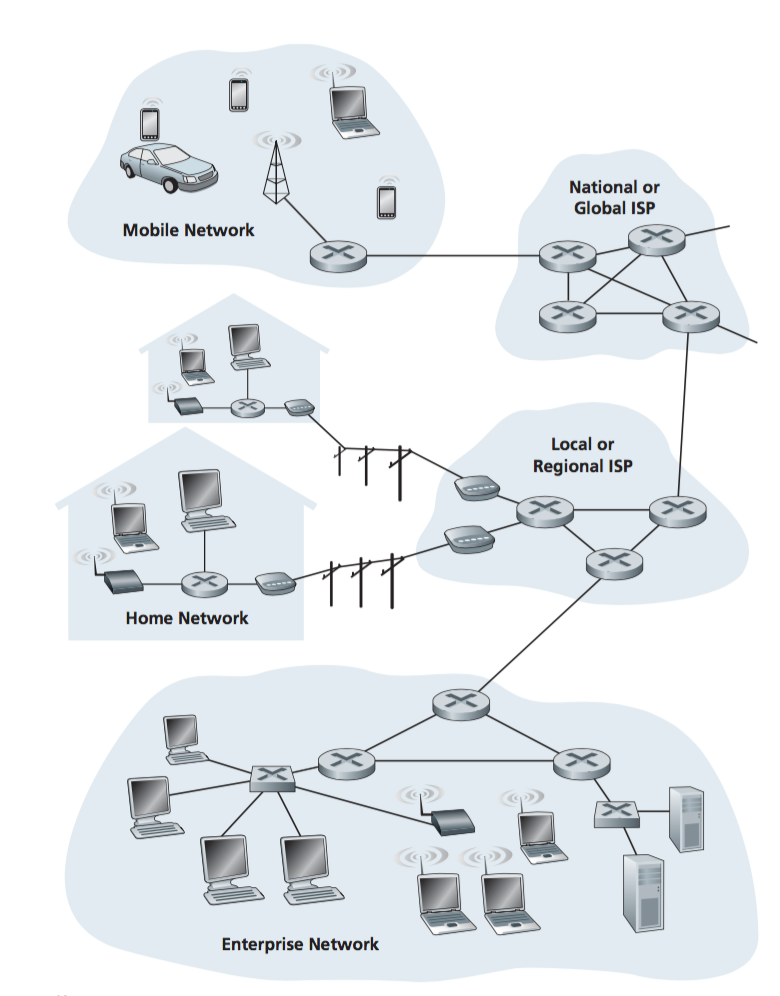
\includegraphics[scale=0.5]{1-networks/internet.png}

\subsection{Home access}
\begin{itemize}
	\item DSL (Digital Subscriber Line)
	\item Cable
	\item FTTH (Fiber To The Home)
	\item Dial-up
	\item Satelite
\end{itemize}

\subsection{Packet switching}
\begin{itemize}
	\item Store-and-forward transmission
	\item Output buffer for hver link
	\item Forwarding table
	\item Queing delays
\end{itemize}

\subsection{Circuit switching}
\begin{itemize}
	\item Reserverer en rute til destinationen (end-to-end)
	\item Ingen delays
\end{itemize}

{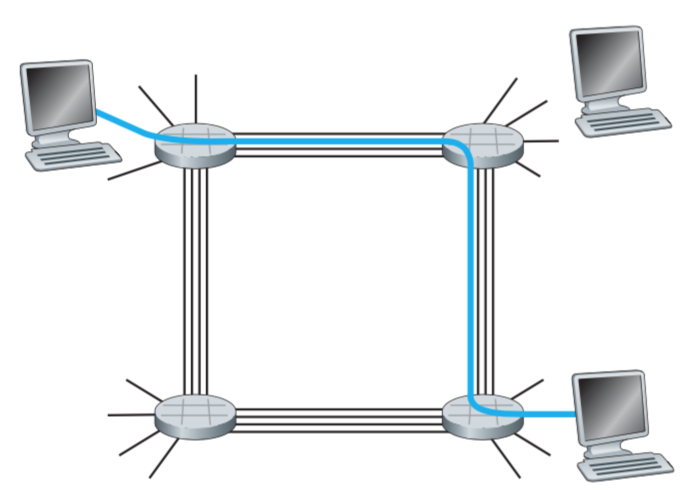
\includegraphics[scale=0.7]{1-networks/circuit-switched-network.png}

\section{Protokol}

\subsection{Hvad er en protokol}
\begin{itemize}
	\item Regelsæt
	\item Definerer måden hvorpå en opgave skal udføres
\end{itemize}

\subsection{Hvad bruger vi protokoller til?}
\begin{itemize}
	\item At have en fælles bestemmelse for hvordan 2 systemer/entiteter kommunikerer, uden de har kendskab til hinandens indre virkener
	\item Mindsker fejlmargin
\end{itemize}

{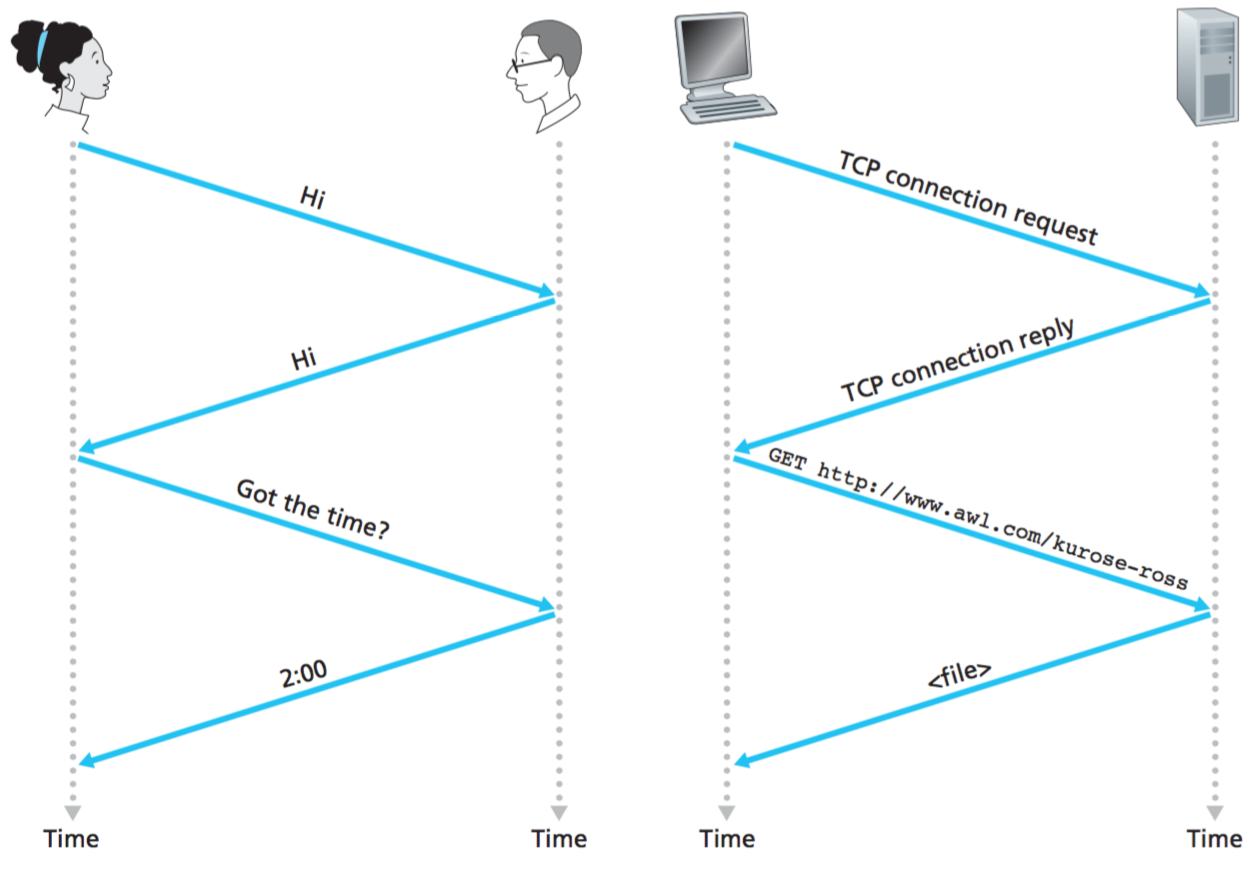
\includegraphics[scale=0.7]{1-networks/protokol.png}

\subsection{Protokoller}
\begin{itemize}
	\item IP
	\item TCP
	\item UDP
	\item HTTP(S)
	\item FTP(S)
	\item SMTP
	\item ...
\end{itemize}

\section{Netværkslag}

\subsection{Modeller}
\begin{itemize}
	\item Fem-lags internet protokol stack
	\item Syv-lags ISO (International Standards Organization) OSI (Open Systems Interconnection) model
\end{itemize}

{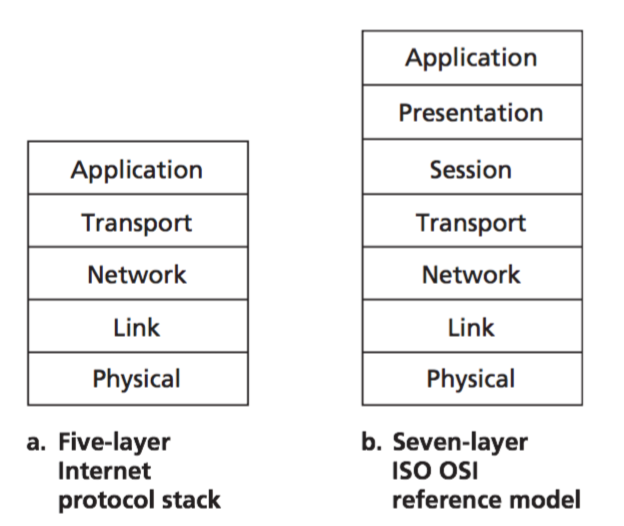
\includegraphics[scale=1]{1-networks/netvaerkslag.png}

\chapter{Application layer: HTTP, FTP, SMTP, DNS}
\section{Introduktion}
\begin{itemize}
	\item Kommunikation mellem processor på 2 seperate end systems
	\item Klient
	\item Server
	\item En process kan være både klient og server (ex. P2P)
\end{itemize}

\section{Arkitekturer i netværksapplikationer}
\begin{itemize}
	\item Klient-server arkitektur
	\item Peer-to-peer (P2P) arkitektur
\end{itemize}

\section{Protokoller}
\begin{itemize}
	\item Headers \& data
	\item Status koder
\end{itemize}

\subsection{HTTP}
\begin{itemize}
	\item Hypertext Transfer Protocol
	\item Klient ofte en browser
	\item Server er en webserver, ex. Apache
	\item HTML, billeder, video, XML, JSON osv.
	\item Stateless
	\item Cookies
	\item TCP
\end{itemize}

{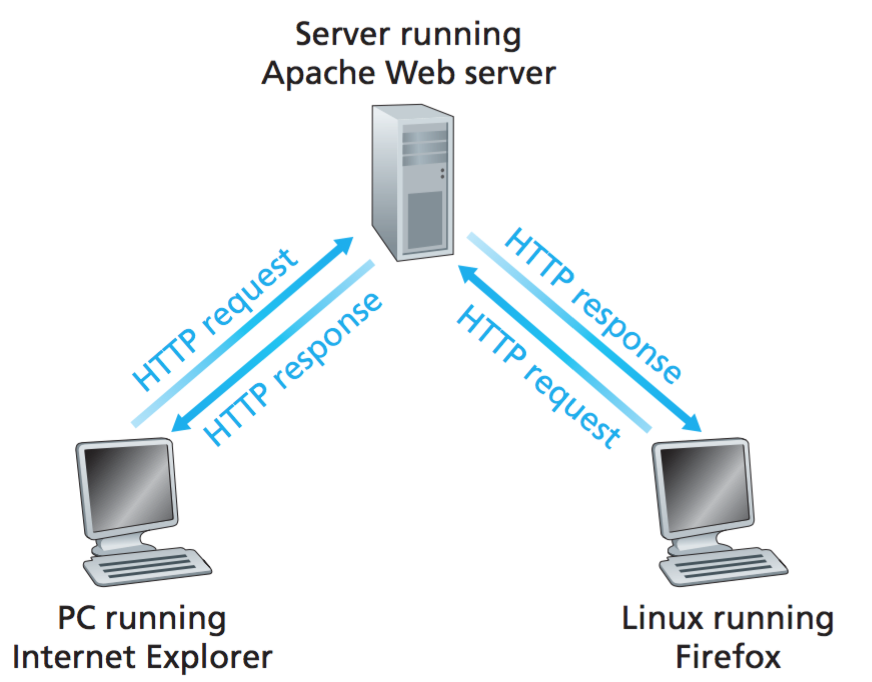
\includegraphics[scale=0.5]{2-application-layer/http-client-server.png}

\textbf{Request}
GET /somedir/page.html HTTP/1.1 \\
Host: www.someschool.edu \\
Connection: close \\
User-agent: Mozilla/5.0 \\
Accept-language: fr \\

\textbf{Response}
HTTP/1.0 200 OK \\
Date: Fri, 31 Dec 1999 23:59:59 GMT \\
Content-Type: text/html \\
Content-Length: 1354

\textless html\textgreater \\
\textless body\textgreater \\
\textless h1\textgreater Hello world!\textless /h1\textgreater \\
… \\
\textless /body\textgreater \\
\textless /html\textgreater \\

\subsection{FTP}
\begin{itemize}
	\item File Transfer Protocol
	\item Port 20 \& 21
	\item Serveren hoster filer
	\item Klienten kan henter filer mm., fra serveren
	\item Kræver ofte verificering med brugernavn og adgangskode
	\item Stateful
\end{itemize}

{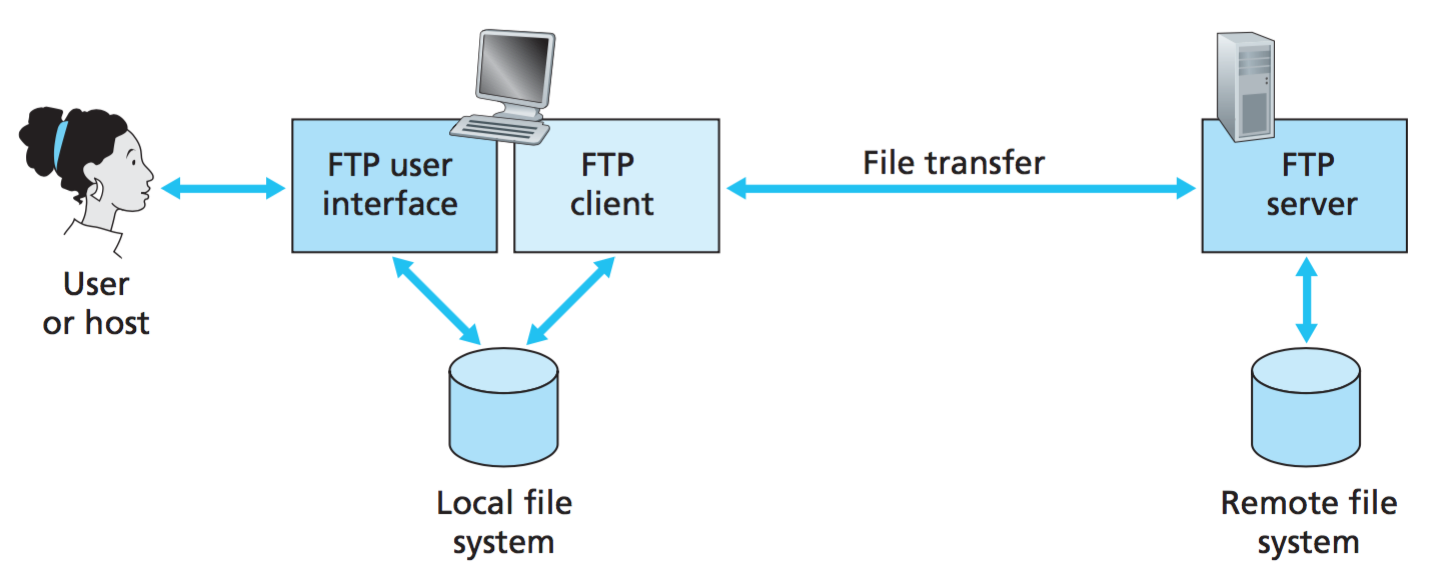
\includegraphics[scale=0.5]{2-application-layer/ftp-client-server.png}

\subsection{SMTP, POP3, IMAP}
\begin{itemize}
	\item Simple Mail Transfer Protocol, Post Office Protocol - Version 3, Internet Message Access Protocol
	\item SMTP sender mail
	\item POP3 \& IMAP tilgår mail
\end{itemize}

\subsection{DNS}
\begin{itemize}
	\item Ofte brugt af andre protokoller i Application-laget (HTTP, SMTP, FTP osv.)
	\item Domain Name System
	\item Distribueret (Decentralized)
	\item Mapper domænenavne til ip-adresser
\end{itemize}

\section{Sockets}
\begin{itemize}
	\item Kommunikation mellem appliktionslaget og transportlaget
	\item UDP
	\item TCP
\end{itemize}

\chapter{Transport layer: TCP, UDP}
\section{Introduktion}
\begin{itemize}
	\item Nice-to-have lag
	\item Sockets bruges til kommunikation med applikationslaget
	\item Laver TCP/UDP pakker med headers
	\item Multiplexing
	\item Demultiplexing
\end{itemize}

{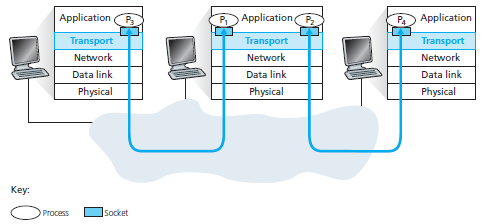
\includegraphics{3-transport-layer/transport-layer-sockets.png}

\section{TCP}
\begin{itemize}
	\item Transmission Control Protocol
	\item Connection orienteret
	\item 3-way-handshake
	\item Maksimal pakkestørrelse på64 kBytes, men bruger som regel 1500 bytes
	\item Identificeres ved et socket par (IP1:80,IP1:81)
	\item Bytestream
	\item Pålidelig
	\item Flow control
	\item Congestion handling
\end{itemize}

{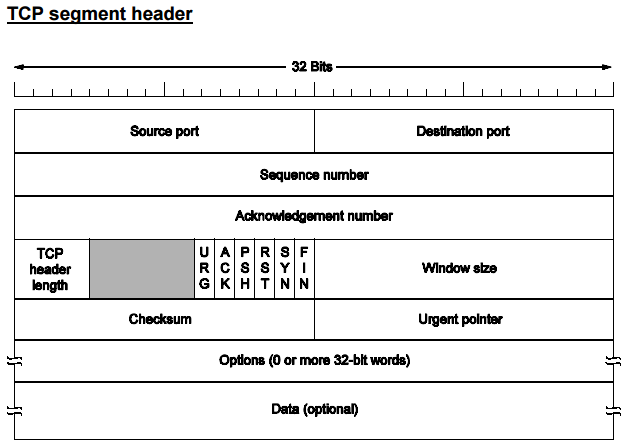
\includegraphics{3-transport-layer/tcp-header.png}

\section{UDP}
\begin{itemize}
	\item User Datagram Protocol
	\item Connection-less
	\item Ip datagram med en lille UDP header
	\item Upålidelig
\end{itemize}

{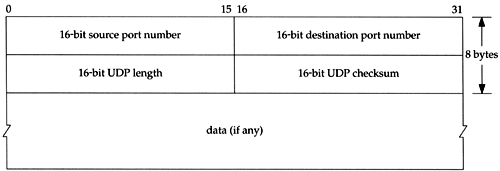
\includegraphics{3-transport-layer/udp-header.png}

\section{Brug af protokoller}

{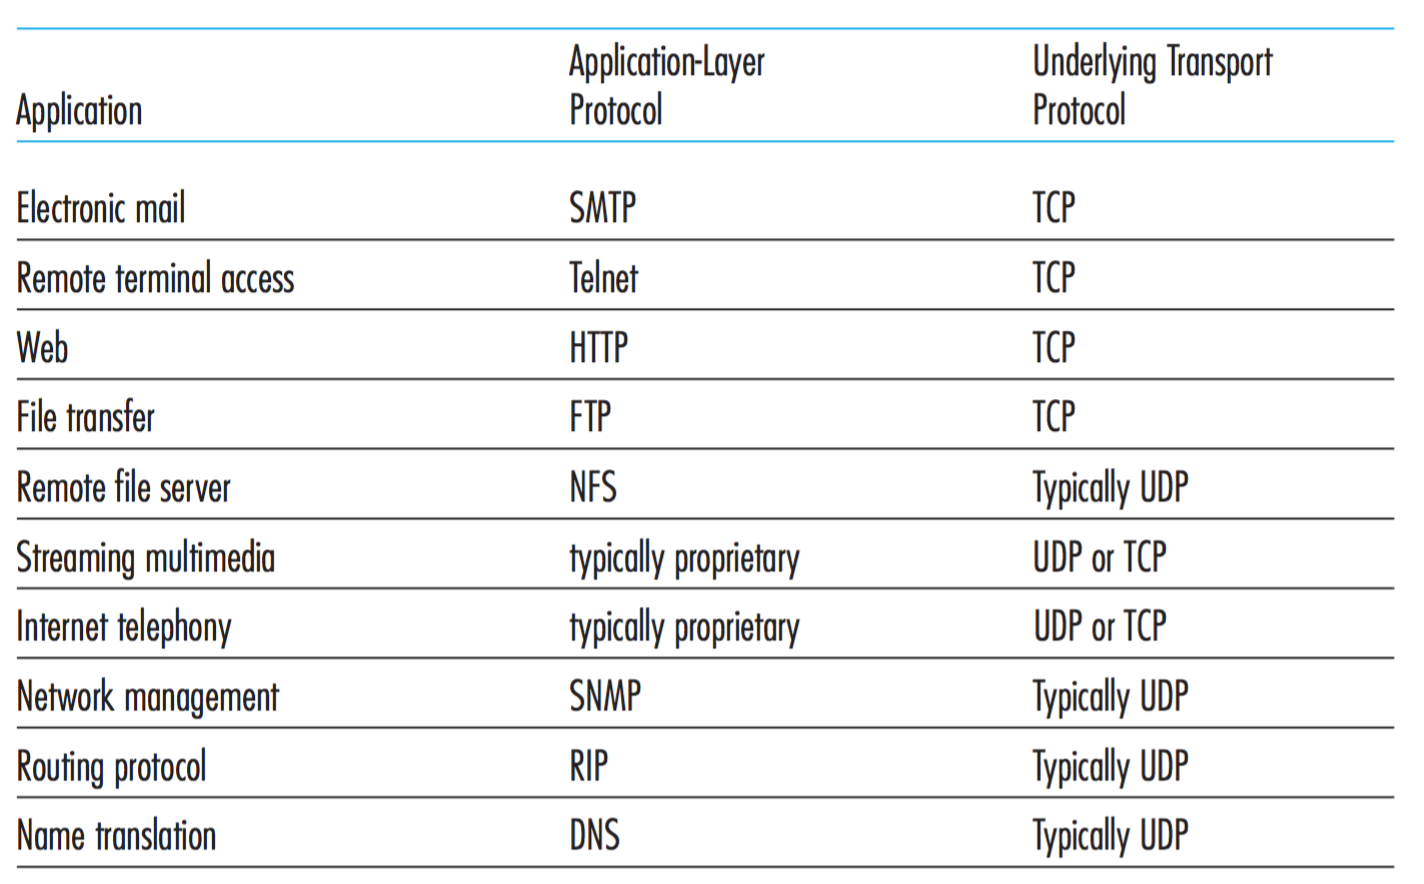
\includegraphics[scale=0.6]{3-transport-layer/brug-af-protokoller.png}

\chapter{Network layer: IP, Routing algorithms}
\section{Introduktion}
Netværklaget omhandler en host-to-host kommunikation service dvs. dens opgave består i at sende pakker fra en ‘sending host’ til en ‘receiving host’.
\begin{center}
  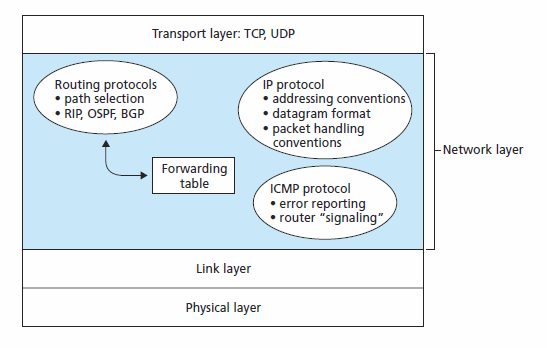
\includegraphics{4-network-layer/networklayer.png}
\end{center}
\begin{itemize}
	\item Står for addressering
	\item Leverer pakker til applikationer.
	\item Routing
	\item Forwarding 
	\item Modtager segmenter fra transportlag -> indkapsler dette i datagram (+IP) -> Videre til routeren.
\end{itemize}

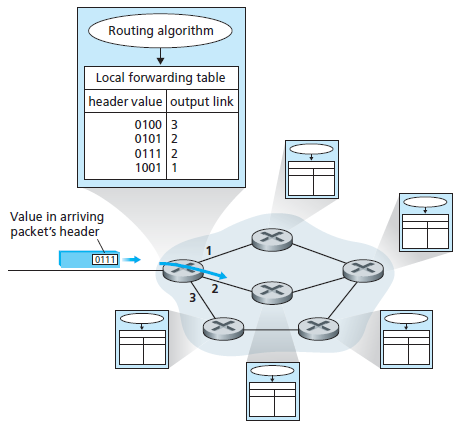
\includegraphics{4-network-layer/RoutingForwardring.png}

\subsection{Forwarding}
\begin{itemize}
\item Ankommen pakke i router skal flyttes til udgående link (Videre på netværk/Tilkoblet klient på router)
\item Forwardring tabel
\item Analyserer bestemt field (header).
\item Bruges til at indeksere i forwarding tabel.
\end{itemize}

\subsection{Routing}
\begin{itemize}
\item Finde vej ved hjælp af routing protokoller.
\item Stibestemmelse
\item Routing Algoritmer
\end{itemize}

\section{Services på netværkslaget}
\begin{itemize}
\item Guaranteed delivery (Garanti for pakkes ankomst ved destination) + bounded delay.
\item In-order-packet-delivery (Ankommer i rækkefølgen de blev sendt).
\item Security Services (Kryptering af datagrammer)
\item Osv.
\end{itemize}

\section{Virtuelle kredsløb og datagramnetværk}
\subsection{Virtuelle kredsløb}
{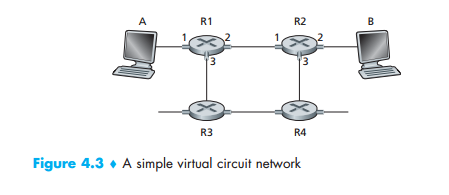
\includegraphics{4-network-layer/vc-network.png}
\begin{itemize}
	\item 1) Rute (En række routere og links). 
	\item 2) VC-nummer (Ét nummer for hver link langs en rute)
	\item 3) Indgange i FW-table i hver router land en Route
	\item Videresendelsestabel
	\item Opbevarer oplysninger om forbindelsesstatus.
\end{itemize}

\subsection{Datagramnetværk}
{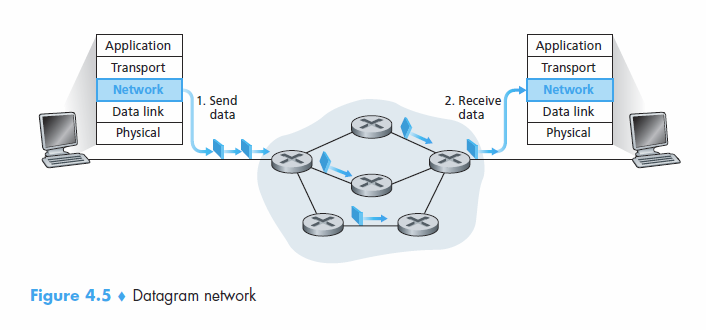
\includegraphics{4-network-layer/datagramnetwork.png}
\begin{itemize}
	\item For hver packetforsendelse - destinations adresse tilføjes og afsendes.
	\item Packet bevæger sig igennem routere mod distination.
	\item Routerne benytter destinationsadressen til at forward. 
	\item Opbevarer INGEN oplysninger om forbindelsesstatus
	\item 32 bit destinationsadresse (IP-Datagram).
\end{itemize}

\section{Sådan virker en router}
En router er en enhed på et computernetværk som forbinder et antal logiske eller fysiske netværk ved at videresende pakker fra et netværk til deres destination på et andet netværk i en process kaldet routing. Routeren arbejder på OSI-modellens lag 3 (netværkslaget), i internetprotokollen kaldes dette lag IP-laget.
\begin{center}
  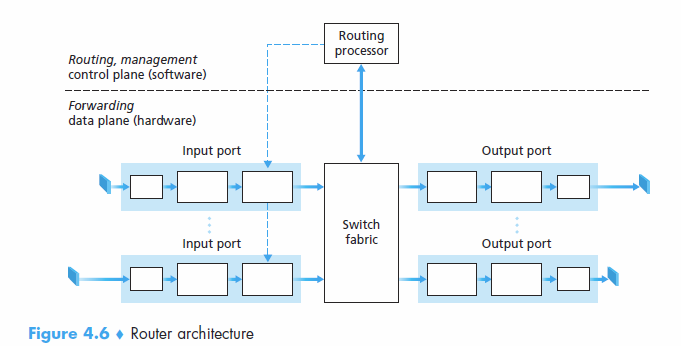
\includegraphics[scale=0.8]{4-network-layer/whats-inside-a-router.png}
\end{center}
\begin{itemize}
	\item Input porte (lookup function - skal en packet sendes igennem denne?)
	\item Switching fabric (Forbinder input/ output porte)
	\item Output porte (Herfra sendes packets - Bidirectional) 
	\item Routing processor (Routing protokoller / states på links)
\end{itemize}


{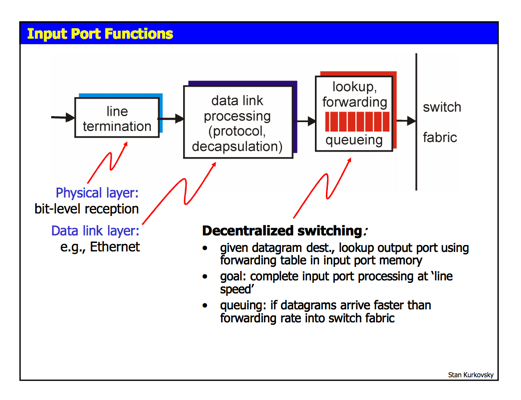
\includegraphics{4-network-layer/router-input-port}
{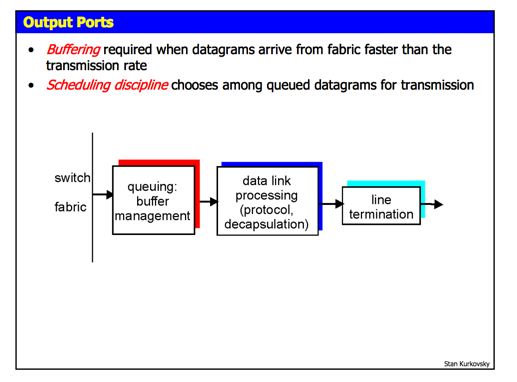
\includegraphics{4-network-layer/router-output-port.png}

\section{Internetprotokollen – IP}
Den protokol der bruges på internettets netværkslag er IP protokollen. 
Derfor kaldes internettets netværkslag også for IP-laget. Internetprotokollen er imidlertid bare en del af internettets netværkslag, der består af 3 hovedkomponenter.
\begin{center}
  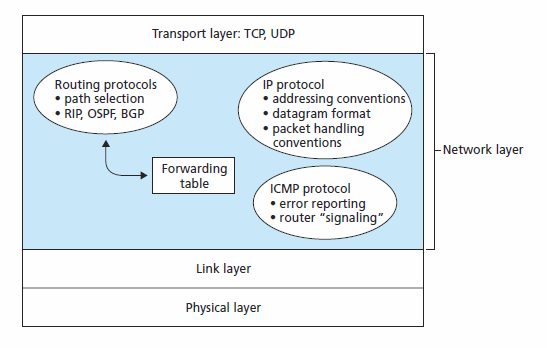
\includegraphics{4-network-layer/networklayer.png}
\end{center}
\begin{itemize}
	\item Internet Protocol(adressering - felter i datagrammet - IPv4 - IPv6)
	\item Stibestemmelse(beregne pakkes sti - vedligeholdelse af netværket)
	\item Fejlrapportering(rapportere  fejl i datagrammet - ICMP
\end{itemize}

\section{Ipv4 datagram}
{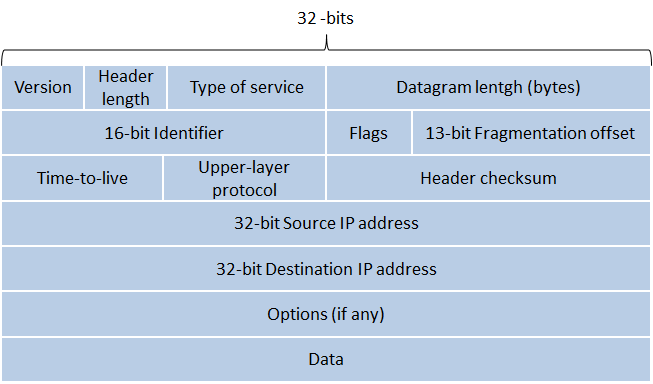
\includegraphics{4-network-layer/IPv4_datagram.png}
\begin{itemize}
	\item Version: (IPv4 / IPv6)
	\item Header length: (Hvor starter dataen?)
	\item Servicetype: (IP-datagram type: Realtime / non-realtime.)
	\item Datagram-length: Datagrammets længde (Header + data)
	\item Identifikation, flag og start på opdeling.
	\item Time-to-live: (Sørger for at datagram ikke lever for evig - counter dekrementeres).
	\item Protokol: TCP eller UDP på transportlag.
	\item Header checksum: Udregnes fra summen af bytes - kontrolleres af modtager.
	\item Source/destination IP address: Afsender og modtageradresse (IP)
	\item Settings: Mulighed for udvidelse af IP header.
	\item Data: Transportlag segmentet (Reel data).
\end{itemize}

\section{IPv4 adressering}
En vært er sædvanligvis koblet til netværket med én forbindelse. Grænsen mellem værten og det fysiske netværk kaldes en interface.
\begin{center}
  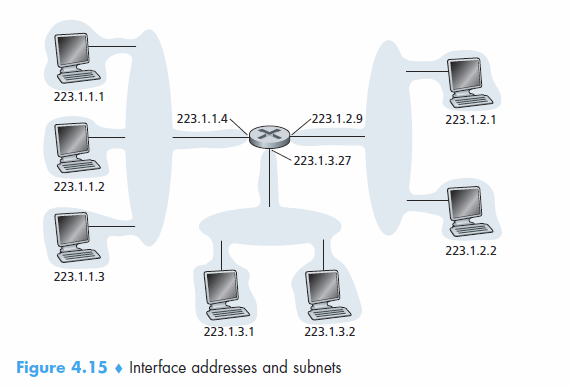
\includegraphics{4-network-layer/ipv4-adressering.png}
\end{center}
\begin{itemize}
	\item Interface (Router har et interface for hvert link.)
 	\item Hvert host og router interface har en IP tilknyttet.
	\item IP adressen knyttet til interfacet
	\item IP addresse 32 bits, dotted decimal format
	\item Flere host interfaces på ét router interface = subnet.
	\item 223.1.1.0/24 - /24 notation = subnet mask.
\end{itemize}

  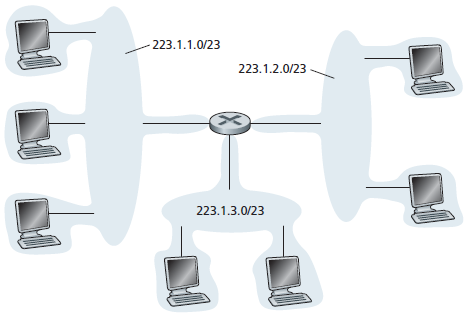
\includegraphics{4-network-layer/ivpsubnet.png}

\section{Hierarkisk routing}
En router er en enhed på et computernetværk som forbinder et antal logiske eller fysiske netværk ved at videresende pakker fra et netværk til deres destination på et andet netværk i en process kaldet routing. Routeren arbejder på OSI-modellens lag 3 (netværkslaget), i internetprotokollen kaldes dette lag IP-laget.
\begin{center}
  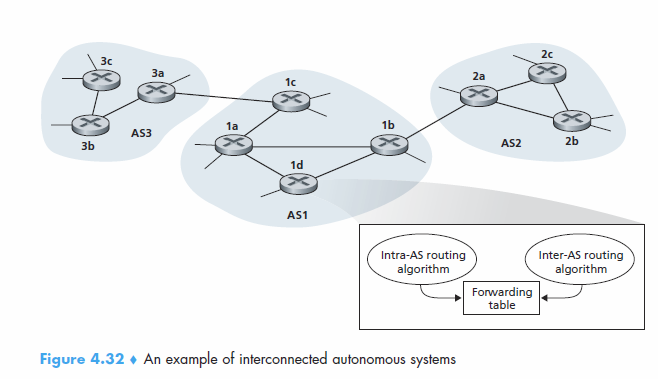
\includegraphics[scale=0.8]{4-network-layer/hierarkisk-routing.png}
\end{center}
\begin{itemize}
	\item Metode til at route i netværk.
	\item Baseret på hierarkisk adressering.
	\item Arrangering af routere i et hierarki. 
\end{itemize}


\section{Tildeling af IP adresser}
\begin{itemize}
	\item Manuel konfiguration
	\item Dynamic Host Configuration Protocol – DHCP(plug-and-play protokol - flere brugere - færre ip adresser - let at administrerer - adressekonflikt)
\end{itemize}


\section{ICMP – Internet Control Message Protocol}
\begin{itemize}
	\item Error reporting
	\item Hvis "Destination network unreachable" fejl modtages = IMCP.
	\item Sti til host kunne ikke findes.
	\item Betragtes som en del af IP - men befinder sig lige over IP.
	\item ICMP beskeder sender i IP datagrammer.
	\item ICMP = IP Payload, ligesom UDP og TCP segmenter.

\end{itemize}
{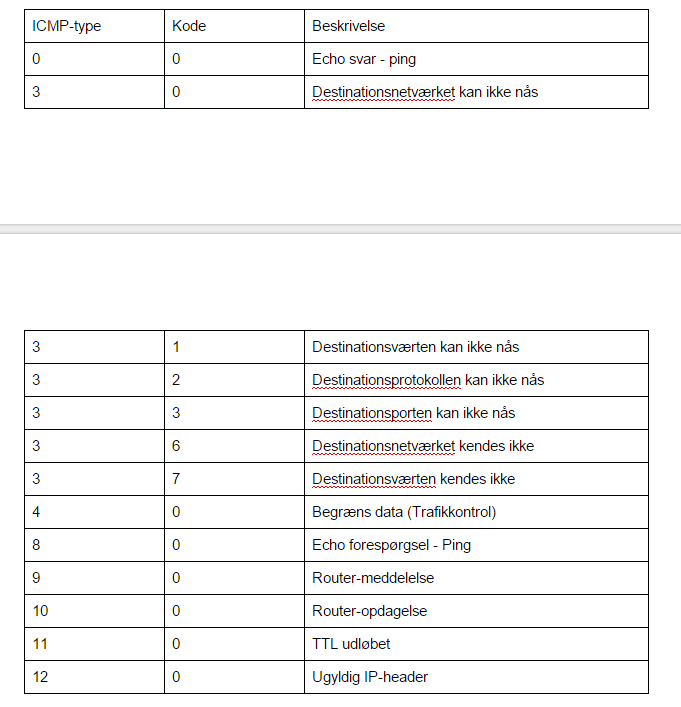
\includegraphics{4-network-layer/icmp-tabel.png}



\chapter{Data link layer: Error \& CRC, LAN, MAC, Ethernet, hubs \& switches}
\section{Introduktion}
\begin{itemize}
	\item Implementeret i network interface card'et (NIC)
	\item Framing
	\item Checksum
	\item Errorhandling (Ethernet vs. WiFi)
	\item Nodes \& links
\end{itemize}

\section{Multiple Access}
\begin{itemize}
	\item Point-to-point link
	\item Broadcast link
	\item Multiple access problemer
\end{itemize}

\subsection{Protokoller}
\begin{itemize}
	\item Channel partitioning protocols (CDMA)
	\item Random access protocols (aloha, slotted aloha, CSMA)
	\item Taking-turns protocols (polling protocol, token-passing protocol)
\end{itemize}

\section{Error detection \& correction}
\begin{itemize}
	\item Checksum: Error detection bits
	\item Modtager kontrollerer frame for fejl
	\item Afhængig af link-lags protokol kasseres eller rettes frames med fejl
\end{itemize}

\section{Link layer addressering}
\subsection{MAC}
\begin{itemize}
	\item Media Access Control
	\item 48 bit MAX adresse (NIC kort)
	\item Administreret af IEEE (the Institue of Electrical and Electronics Engineers)
	\item Flytbar
\end{itemize}

{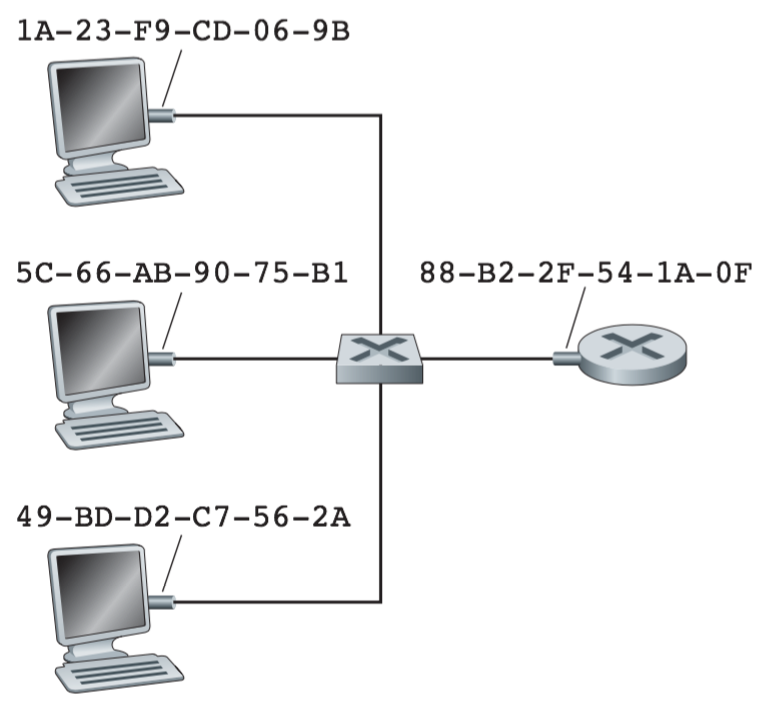
\includegraphics{5-data-link-layer/mac.png}

\subsection{ARP}
\begin{itemize}
	\item Address Resolution Protocol
	\item Mapper ip-addresser til MAC adresser
\end{itemize}

{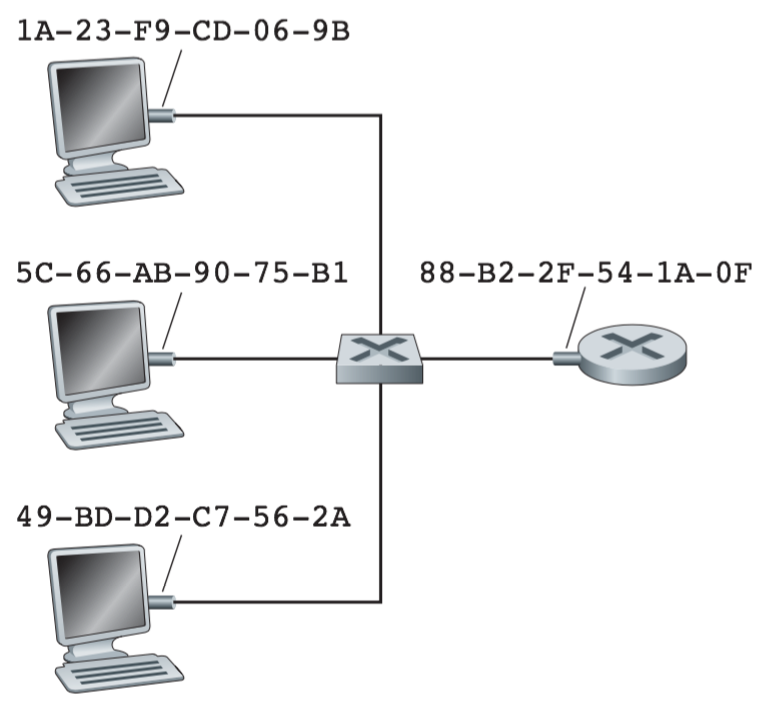
\includegraphics{5-data-link-layer/mac.png}

\section{Ethernet}
\begin{itemize}
	\item Mest udbredte LAN teknologi
	\item Frame struktur
\end{itemize}

{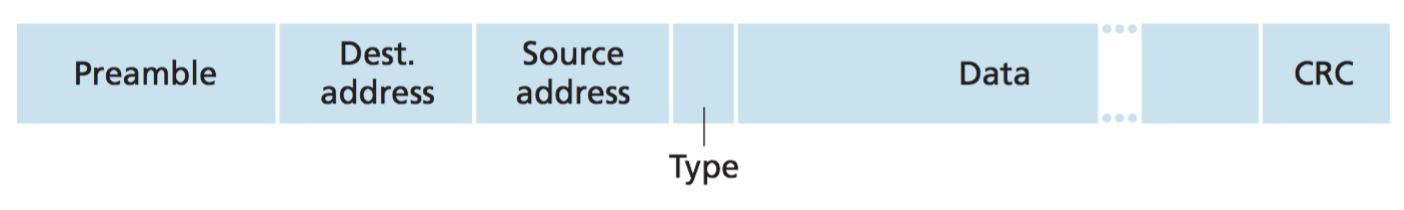
\includegraphics[scale=0.6]{5-data-link-layer/ethernet.png}

\chapter{Wireless: CDMA, MACAW, 802.11, overview: Bluetooth and 802.16}
\section{Introduktion}
\begin{itemize}
	\item Base station
	\item End systems
	\item Dækning
	\item 802.11 protokollen
\end{itemize}

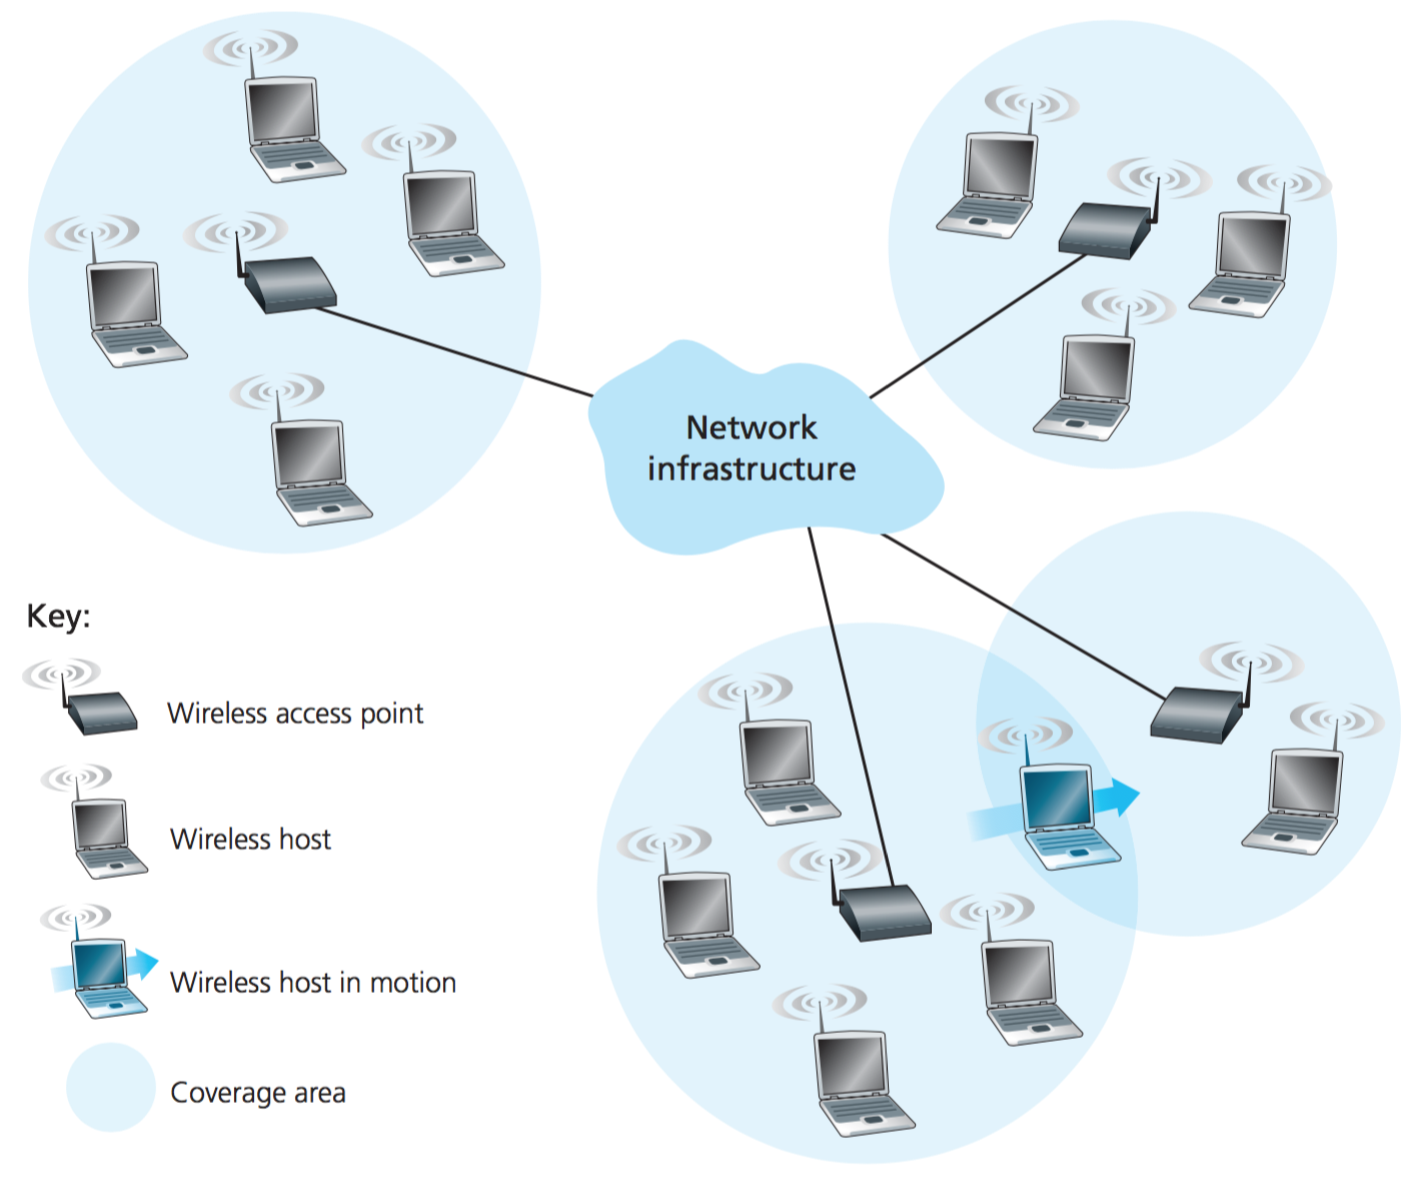
\includegraphics[scale=0.6]{6-wireless/wireless-network.png}

\section{Ulemper ved WiFi}
\begin{itemize}
	\item Svækket styrke hvis signalet skal passere igennem objekter/vægge osv
	\item Forstyrrelser fra andre kilder på samme frekvensbånd (telefoner, mikrobølgeovne)
	\item Multipath propagation: Signal reflekteres 
	\item Disse svagheder resulterer i bit errors
\end{itemize}

\section{Bit Errors}
\begin{itemize}
	\item SNR = Signal-to-Noise Ratio, måles i dB
	\item BER = Bit Error Rate
	\item Højere SNR = lavere BER
\end{itemize}

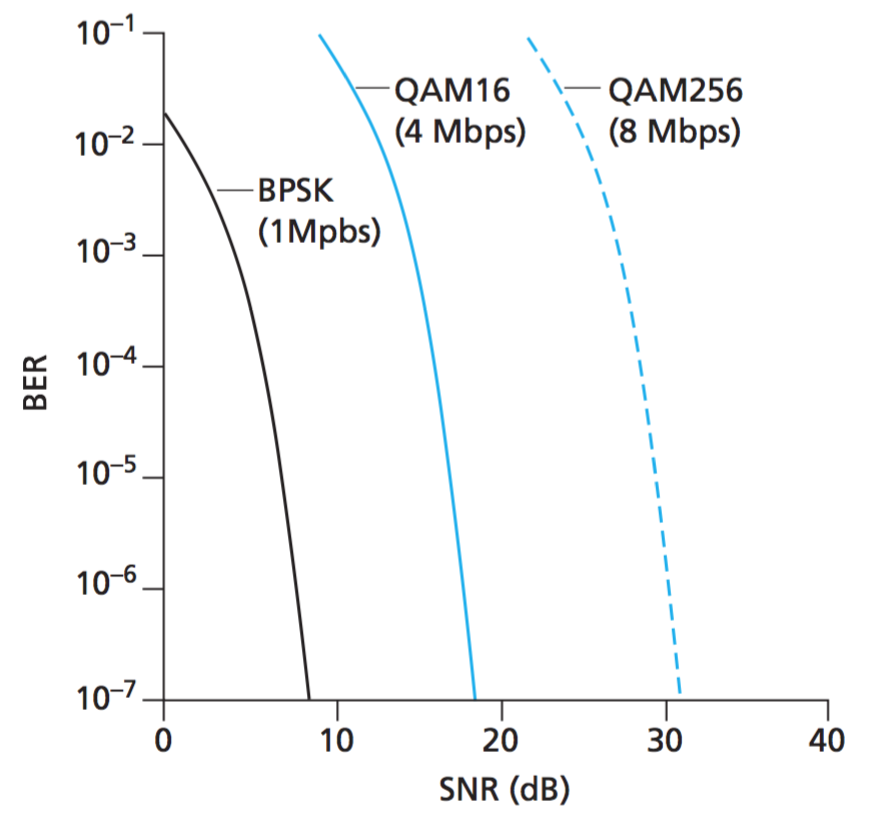
\includegraphics[scale=0.6]{6-wireless/snr-to-ber.png}

\section{Multiple Access}
\begin{itemize}
	\item Channel partitioning protocols - CDMA (Code Division Multiple Access)
	\item Random access protocols - CSMA
	\item Taking-turns protocols
	\item 802.11 bruger CSMA/CA - Collision Avoidance, Ethernet = Collision Detection
\end{itemize}

\chapter{Security overview: Authentication, integrity, encryption \& keys}
Handler om at sikre de data der sendes mellem systems på LAN netværk og internettet, så det ikke kan læses af uvedkommende.

\section{Kryptografi}
\begin{itemize}
	\item Plaintext/cleartext = Ukrypteret besked
	\item Ciphertext = Krypteret besked
\end{itemize}


\subsection{Symmetrisk}
\begin{itemize}
	\item Samme nøgle benyttes til kryptering/dekryptering.
	\item Caesar Cipher
	\item Monoalphabetic cipher
\end{itemize}

{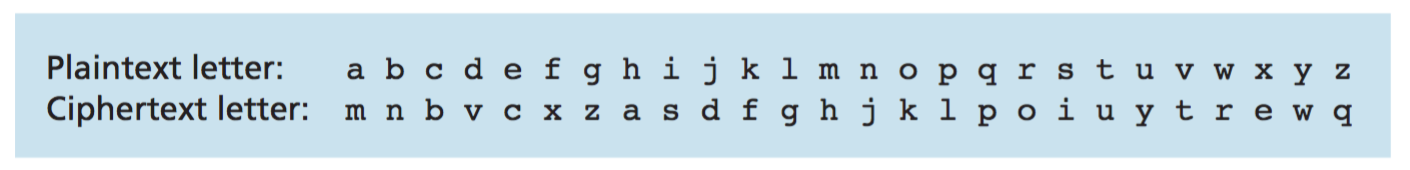
\includegraphics[scale=0.7]{8-security-overview/monoalphabetic.png}

\subsection{Asymmetrisk}
\begin{itemize}
	\item RSA Algoritmen (Navngivet efter opfinderne.)
	\item Private key / public key.
\end{itemize}

{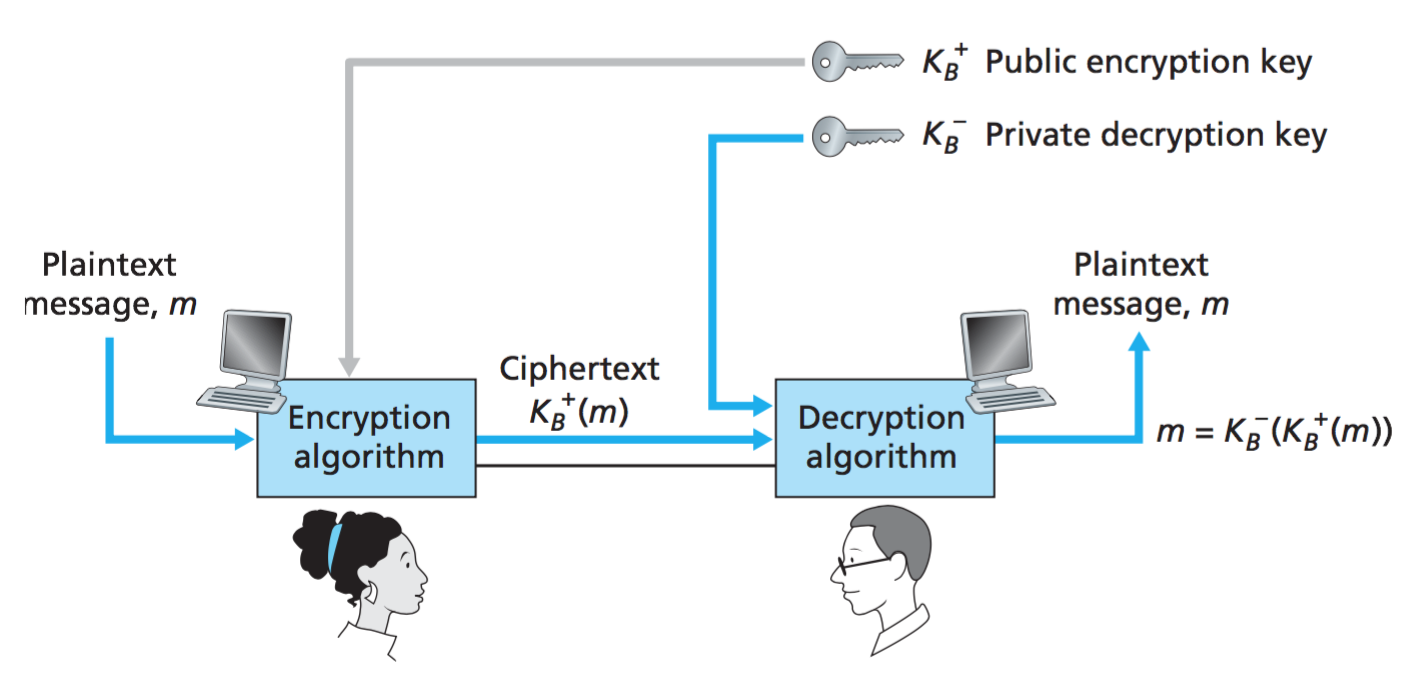
\includegraphics[scale=0.7]{8-security-overview/public-key-cryptography.png}


\subsection{Integritet}
\begin{itemize}
	\item Verificere at beskeden kommer fra den korrekte afsender.
	\item Verificere at beskeden ikke er blevet manipuleret undervejs.
\end{itemize}

\subsection{Hashing}
\begin{itemize}
	\item Vis størrelse er foretrukken for at undgå hashing kollision.
	\item Det skal ikke kunne betale sig, at forsøge at knække koden.
\end{itemize}

\subsection{Digital Signatur}
\begin{itemize}
	\item En digital erstatning for den fysiske signatur.
	\item Benytter public key kryptografi.
\end{itemize}
{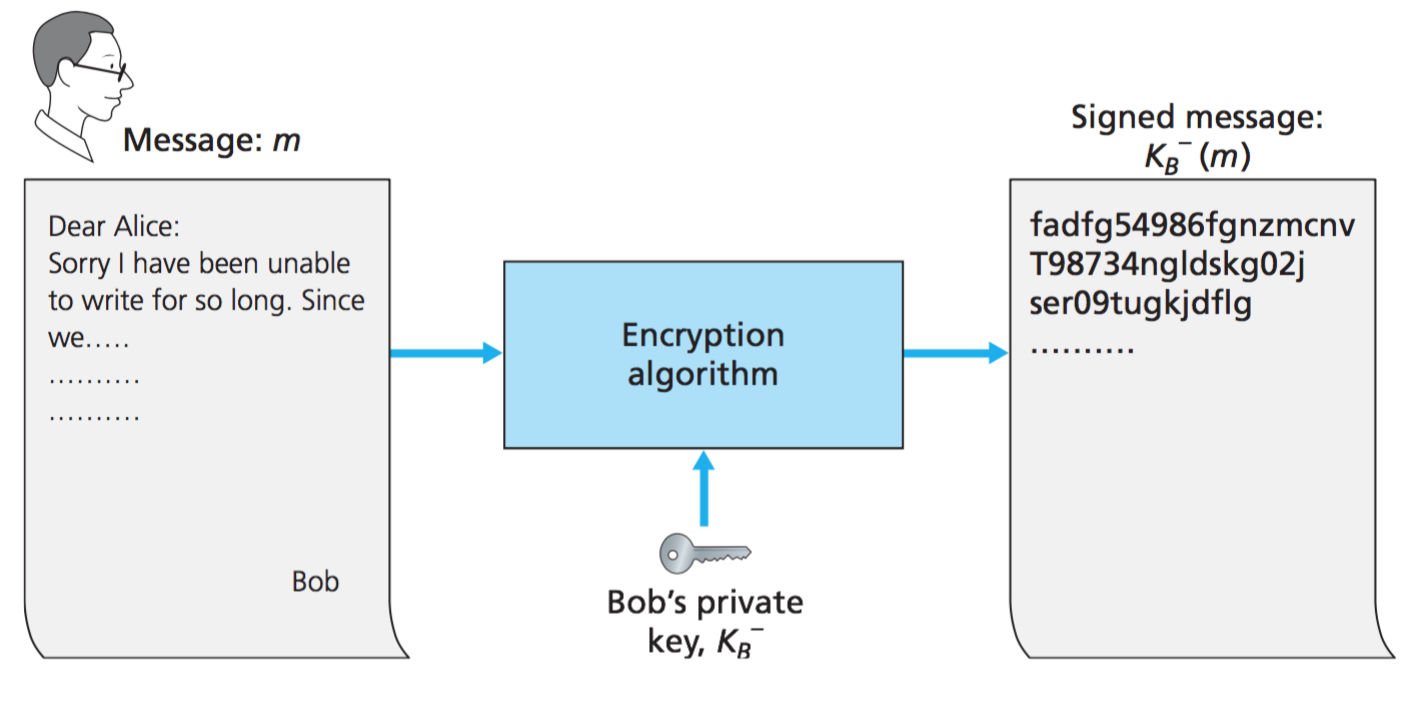
\includegraphics[scale=0.7]{8-security-overview/digital-signature.png}

\subsection{End-point authentication}
\begin{itemize}
	\item En entitet beviser dens identitet overfor en anden entitet på et computer netværk.
	\item Fx: bruger beviser identitet overfor en mailserver.
\end{itemize}

{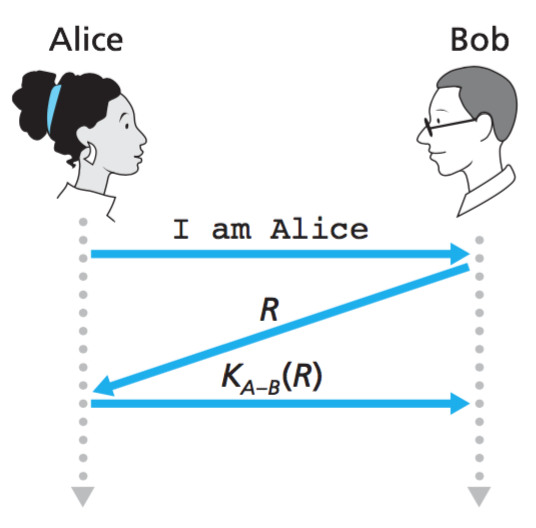
\includegraphics[scale=0.9]{8-security-overview/endpoint.png}

\subsection{SSL}

\begin{itemize}
	\item Kryptografi kan forbedre TCP med henblik på sikkerhedsmæssige aspekter.
	\item Fortrolighed, data-integritet og end point authentication.
	\item Certifikat købes igennem en 3.partsudbyder og installeres på webserver. Består af en public og private key.
	\item TLS (Transport Layer Security) er en modificeret version af SSL.
\end{itemize}

\subsection{IPsec}
\begin{itemize}
	\item IP Security Protocol.
	\item Står for sikkerhed for netværks lag.
	\item Verificering/Kryptering af hver IP-datagram.
	\item Beskytter data flows mellem et host-par: (Host-to-Host, network-to-host, network-to-network).
\end{itemize}



\end{document}